\documentclass{article}

\usepackage{amsthm}
\usepackage{amsfonts}
\usepackage{amsmath}
\usepackage{amssymb}
\usepackage{enumitem}
\usepackage{fullpage}
\usepackage[usenames]{color}
\usepackage{hyperref}
  \hypersetup{
    colorlinks = true,
    urlcolor = blue,       % color of external links using \href
    linkcolor= blue,       % color of internal links 
    citecolor= blue,       % color of links to bibliography
    filecolor= blue,        % color of file links
    }
    
\usepackage{listings}
\usepackage{qtree}
\usepackage{tikz-qtree}

\definecolor{dkgreen}{rgb}{0,0.6,0}
\definecolor{gray}{rgb}{0.5,0.5,0.5}
\definecolor{mauve}{rgb}{0.58,0,0.82}

\lstset{frame=tb,
  language=haskell,
  aboveskip=3mm,
  belowskip=3mm,
  showstringspaces=false,
  columns=flexible,
  basicstyle={\small\ttfamily},
  numbers=none,
  numberstyle=\tiny\color{gray},
  keywordstyle=\color{blue},
  commentstyle=\color{dkgreen},
  stringstyle=\color{mauve},
  breaklines=true,
  breakatwhitespace=true,
  tabsize=3
}

\theoremstyle{theorem} 
   \newtheorem{theorem}{Theorem}[section]
   \newtheorem{corollary}[theorem]{Corollary}
   \newtheorem{lemma}[theorem]{Lemma}
   \newtheorem{proposition}[theorem]{Proposition}
\theoremstyle{definition}
   \newtheorem{definition}[theorem]{Definition}
   \newtheorem{example}[theorem]{Example}
\theoremstyle{remark}    
  \newtheorem{remark}[theorem]{Remark}


\title{CPSC-354 Report}
\author{Eleas Vrahnos  \\ Chapman University}

\date{\today}

\begin{document}

\maketitle

\begin{abstract}
To be written at a later date. 
\end{abstract}

\tableofcontents

\section{Introduction}\label{intro}

This report is written by Eleas Vrahnos. It details all assignments and progress made in the Programming Languages course at Chapman University. It includes weekly homework assigments, programming assignments, and a final project that demonstrate understanding and application in various class topics.

\section{Homework}\label{homework}

This section will contain my solutions to the weekly homework assignments. 

\subsection{Week 1}

The following is a Python implementation of the Euclidean algorithm:

\begin{lstlisting}[language=Python]
def gcd(a,b):
    while a != b:
        if a > b:
            a = a-b
        else:
            b = b-a
    return a
\end{lstlisting}

\newpage % Temporary page break

\noindent We can test this code by going through the function with a sample input \texttt{gcd(9, 33)}, step by step.

\begin{enumerate}[noitemsep]
  \item \texttt{gcd(9, 33)}
  \begin{itemize}
      \item The function is called, assigning 9 to variable \texttt{a} and 33 to variable \texttt{b}.
  \end{itemize} 
  \item \texttt{while a != b:}
  \begin{itemize}
      \item The while loop condition returns True, so the loop starts.
  \end{itemize}
  \item \texttt{else:}
  \begin{itemize}
      \item \texttt{a > b} (9 $>$ 33) returns False, so the else block executes.
  \end{itemize}
  \item \texttt{b = b-a}
  \begin{itemize}
      \item \texttt{b} is now assigned to $33 - 9$, which is $24$.
  \end{itemize}
  \item \texttt{while a != b:}
  \begin{itemize}
      \item The while loop condition returns True, so the loop starts.
  \end{itemize}
  \item \texttt{else:}
  \begin{itemize}
      \item \texttt{a > b} (9 $>$ 24) returns False, so the else block executes.
  \end{itemize}
  \item \texttt{b = b-a}
  \begin{itemize}
      \item \texttt{b} is now assigned to $24 - 9$, which is $15$.
  \end{itemize}
  \item \texttt{while a != b:}
  \begin{itemize}
      \item The while loop condition returns True, so the loop starts.
  \end{itemize}
  \item \texttt{else:}
  \begin{itemize}
      \item \texttt{a > b} (9 $>$ 15) returns False, so the else block executes.
  \end{itemize}
  \item \texttt{b = b-a}
  \begin{itemize}
      \item \texttt{b} is now assigned to $15 - 9$, which is $6$.
  \end{itemize}
  \item \texttt{while a != b:}
  \begin{itemize}
      \item The while loop condition returns True, so the loop starts.
  \end{itemize}
  \item \texttt{if a > b:}
  \begin{itemize}
      \item \texttt{a > b} (9 $>$ 6) returns True, so the first block executes.
  \end{itemize}
  \item \texttt{a = a-b}
  \begin{itemize}
      \item \texttt{a} is now assigned to $9 - 6$, which is $3$.
  \end{itemize}
  \item \texttt{while a != b:}
  \begin{itemize}
      \item The while loop condition returns True, so the loop starts.
  \end{itemize}
  \item \texttt{else:}
  \begin{itemize}
      \item \texttt{a > b} (3 $>$ 6) returns False, so the else block executes.
  \end{itemize}
  \item \texttt{b = b-a}
  \begin{itemize}
      \item \texttt{b} is now assigned to $6 - 3$, which is $3$.
  \end{itemize}
  \item \texttt{while a != b:}
  \begin{itemize}
      \item The while loop condition returns False (\texttt{3 == 3}), so the loop ends.
  \end{itemize}
  \item \texttt{return a}
  \begin{itemize}
      \item \texttt{a} is returned from the function, giving the correct greatest common divisor of \textbf{3}.
  \end{itemize}
\end{enumerate}
\subsection{Week 2}


The following are implementations of various functions in Haskell. \newline

% select_evens function
\noindent \texttt{select\_evens}, lists the even-indexed elements of a given list:
\begin{lstlisting}[language=Haskell]
-- Implementation
select_evens [] = [] -- in the case of a list with even number elements
select_evens (x:[]) = [] -- in the case of a list with odd number elements
select_evens (x:y:xs) = y : select_evens (xs)

-- Execution Sequence with example ["a","b","c","d","e"]
select_evens ["a","b","c","d","e"] =
    "b" : (select_evens["c","d","e"]) = 
    "b" : ("d" : (select_evens["e"])) =
    "b" : ("d" : ([])) = 
    ["b","d"]
\end{lstlisting} 

% select_odds function
\noindent \texttt{select\_odds}, lists the odd-indexed elements of a given list:
\begin{lstlisting}[language=Haskell]
-- Implementation
select_odds [] = [] -- in the case of a list with even number elements
select_odds (x:[]) = [x] -- in the case of a list with odd number elements
select_odds (x:y:xs) = x : select_odds (xs)

-- Execution Sequence with example ["a","b","c","d","e"]
select_odds ["a","b","c","d","e"] =
    "a" : (select_odds["c","d","e"]) = 
    "a" : ("c" : (select_odds["e"])) =
    "a" : ("c" : ("e")) = 
    ["a","c","e"]
\end{lstlisting}

% member function
\noindent \texttt{member}, determines whether an element is part of a given list:
\begin{lstlisting}[language=Haskell]
-- Implementation
member a [] = False
member a (x:xs)
    | a==x = True
    | otherwise = member a (xs)

-- Execution Sequence with example 2 [5,2,6]
member 2 [5,2,6] =
    member 2 [2,6] = 
    True
\end{lstlisting}

\newpage % Temporary page break

% append function
\noindent \texttt{append}, appends a list to another list:
\begin{lstlisting}[language=Haskell]
-- Implementation
append [] ys = ys
append (x:xs) ys = x : append xs ys

-- Execution Sequence with example [1,2] [3,4,5]
append [1,2] [3,4,5] =
    1 : (append [2] [3,4,5]) = 
    1 : (2 : (append [] [3,4,5])) =
    1 : (2 : ([3,4,5])) =
    [1,2,3,4,5]
\end{lstlisting}

% revert function
\noindent \texttt{revert}, reverses a list:
\begin{lstlisting}[language=Haskell]
-- Implementation
revert [] = []
revert (x:xs) = append (revert(xs)) [x]

-- Execution Sequence with example [1,2,3]
revert [1,2,3] =
    append (revert [2,3]) [1] =
    append (append (revert [3]) [2]) [1] =
    append (append (append (revert []) [3]) [2]) [1] =
    append (append (append [] [3]) [2]) [1] =
    append (append [3] [2]) [1] = 
    append (3 : (append [] [2])) [1] =
    append (3 : [2]) [1] =
    append [3,2] [1] =
    3 : (append [2] [1]) =
    3 : (2 : (append [] [1]) =
    3 : (2 : [1]) =
    [3,2,1]
\end{lstlisting}

% less_equal function
\noindent \texttt{less\_equal}, checks if the element in a list is less than or equal to the same-indexed element in another list:
\begin{lstlisting}[language=Haskell]
-- Implementation
less_equal [] [] = True
less_equal (x:xs) (y:ys)
    | x > y = False
    | otherwise = less_equal (xs) (ys)

-- Execution Sequence with example [1,2,3] [2,3,2]
less_equal [1,2,3] [2,3,2] =
    less_equal [2,3] [3,2] = 
    less_equal [3] [2] = 
    False
\end{lstlisting}

\newpage % Temporary page break
\subsection{Week 3}

The following investigates the Tower of Hanoi problem. Here is a given Haskell implementation describing moves in the game, as well as the execution sequence for the test input \texttt{hanoi 5 0 2}.
\begin{lstlisting}[language=Haskell]
-- Implementation
hanoi 1 x y = move x y

hanoi (n+1) x y = 
    hanoi n x (other x y) 
    move x y 
    hanoi n (other x y) y

-- Execution Sequence
hanoi 5 0 2
    hanoi 4 0 1
        hanoi 3 0 2
            hanoi 2 0 1
                hanoi 1 0 2 = move 0 2
                move 0 1
                hanoi 1 2 1 = move 2 1
            move 0 2
            hanoi 2 1 2
                hanoi 1 1 0 = move 1 0
                move 1 2
                hanoi 1 0 2 = move 0 2
        move 0 1
        hanoi 3 2 1
            hanoi 2 2 0
                hanoi 1 2 1 = move 2 1
                move 2 0
                hanoi 1 1 0 = move 1 0
            move 2 1
            hanoi 2 0 1
                hanoi 1 0 2 = move 0 2
                move 0 1
                hanoi 1 2 1 = move 2 1
    move 0 2
    hanoi 4 1 2
        hanoi 3 1 0
            hanoi 2 1 2
                hanoi 1 1 0 = move 1 0
                move 1 2
                hanoi 1 0 2 = move 0 2
            move 1 0
            hanoi 2 2 0
                hanoi 1 2 1 = move 2 1
                move 2 0
                hanoi 1 1 0 = move 1 0
        move 1 2
        hanoi 3 0 2
            hanoi 2 0 1
                hanoi 1 0 2 = move 0 2
                move 0 1
                hanoi 1 2 1 = move 2 1
            move 0 2
            hanoi 2 1 2
                hanoi 1 1 0 = move 1 0
                move 1 2
                hanoi 1 0 2 = move 0 2
\end{lstlisting} 
From this execution, the moves for a 5-ring Tower of Hanoi game can be seen as follows:
\begin{lstlisting}
0->2, 0->1, 2->1, 0->2, 1->0, 1->2, 0->2, 0->1, 2->1, 2->0, 1->0, 2->1, 0->2, 0->1, 2->1, 0->2, 1->0, 1->2, 0->2, 1->0, 2->1, 2->0, 1->0, 1->2, 0->2, 0->1, 2->1, 0->2, 1->0, 1->2, 0->2
\end{lstlisting}

\noindent \textbf{Analysis:} From this computation, the word \texttt{hanoi} appears exactly 31 times in the execution. Based on executions of the game with a different number of starting rings, the formula $2^n - 1$ can be derived to determine how many times \texttt{hanoi} will appear, with \texttt{n} being the number of disks in the game.
\subsection{Week 4}
The following compares concrete and abstract syntax trees of various mathematical expressions.

The expression $2+1$:\newline

\hfil
\begin{tikzpicture}
\begin{scope}
\Tree[.Exp [.Exp [.Exp1 [.Exp2 $3$ ]]]
           [.+ ]
           [.Exp1 [.Exp2 $1$ ]]]
\end{scope}
\begin{scope}[xshift=5cm]
\Tree[.Plus [.2 ]
            [.1 ]]
\end{scope}
\end{tikzpicture}
\hfil

The expression $1+2*3$:\newline

\hfil
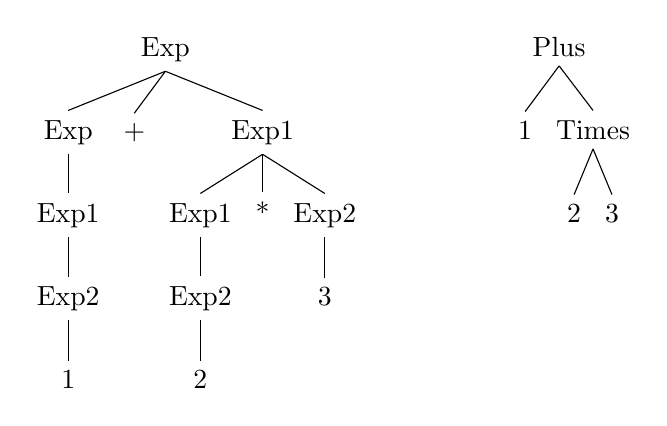
\begin{tikzpicture}
\begin{scope}
\Tree[.Exp [.Exp [.Exp1 [.Exp2 $1$ ]]]
           [.+ ]
           [.Exp1 [.Exp1 [.Exp2 $2$ ]]
                  [.* ]
                  [.Exp2 $3$ ]]]
\end{scope}

\begin{scope}[xshift=5cm]
\Tree[.Plus [.1 ]
            [.Times [.2 ]
                    [.3 ]]]
\end{scope}
\end{tikzpicture}
\hfil

\newpage
The expression $1+(2*3)$:\newline

\hfil
\begin{tikzpicture}
\begin{scope}
\Tree[.Exp [.Exp [.Exp1 [.Exp2 $1$ ]]]
           [.+ ]
           [.Exp1 [.Exp2 [.( ]
                         [.Exp [.Exp1 [.Exp1 [.Exp2 $1$ ]]
                                      [.* ]
                                      [.Exp2 $3$ ]]]
                         [.) ]]]]
                         
\end{scope}

\begin{scope}[xshift=5cm]
\Tree[.Plus [.1 ]
            [.Times [.2 ]
                    [.3 ]]]
\end{scope}
\end{tikzpicture}
\hfil    

The expression $(1+2)*3$:\newline

\hfil
\begin{tikzpicture}
\begin{scope}
\Tree[.Exp [.Exp1 [.Exp1 [.Exp2 [.( ]
                                [.Exp [.Exp [.Exp1 [.Exp2 $1$ ]]]
                                      [.+ ]
                                      [.Exp1 [.Exp2 $2$ ]]]
                                [.) ]]]
           [.* ]
           [.Exp2 $3$ ]]]
                         
\end{scope}

\begin{scope}[xshift=5cm]
\Tree[.Times [.Plus [.1 ]
                    [.2 ]]
             [.3 ]]
\end{scope}
\end{tikzpicture}
\hfil

\newpage
The expression $1+2*3+4*5+6$:\newline

\hfil
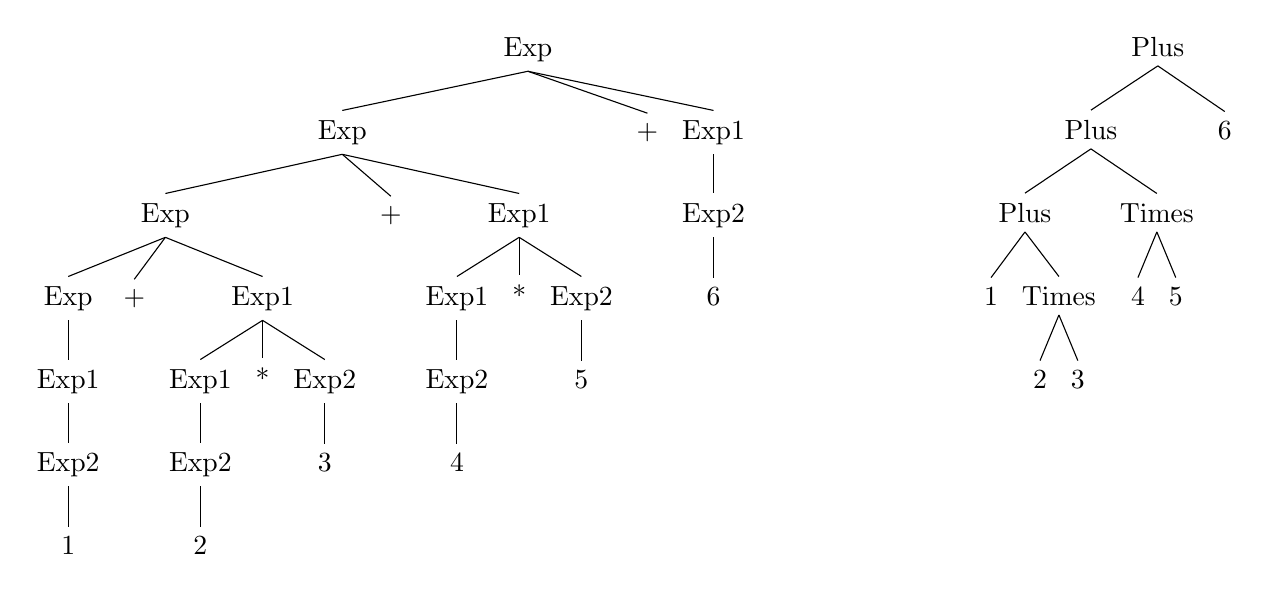
\begin{tikzpicture}
\begin{scope}
\Tree[.Exp [.Exp [.Exp [.Exp [.Exp1 [.Exp2 $1$ ]]]
                       [.+ ]
                       [.Exp1 [.Exp1 [.Exp2 $2$ ]]
                              [.* ]
                              [.Exp2 $3$ ]]]
                 [.+ ]
                 [.Exp1 [.Exp1 [.Exp2 $4$ ]]
                        [.* ]
                        [.Exp2 $5$ ]]]
           [.+ ]
           [.Exp1 [.Exp2 $6$ ]]]
                

                         
\end{scope}

\begin{scope}[xshift=8cm]
\Tree[.Plus [.Plus [.Plus [.1 ]
                          [.Times [.2 ]
                                  [.3 ]]]
                   [.Times [.4 ]
                           [.5 ]]]
            [.6 ]]

                   
\end{scope}
\end{tikzpicture}
\hfil

\noindent \textbf{Analysis of the abstract syntax tree of $1+2+3$}:
The abstract syntax tree of $1+2+3$ would match the tree of $(1+2)+3$. This is because the first breakdown of $+$ separates it to \texttt{Exp} and \texttt{Exp1}, and \texttt{Exp1} cannot reduce down to another sum. Therefore, the right side of the tree must become an integer, while the left side reduces down to a sum. The resulting tree would be as follows, which matches $(1+2)+3$ and not $1+(2+3)$.

\hfil
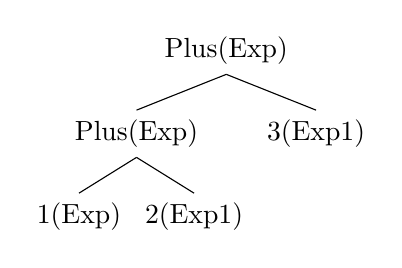
\begin{tikzpicture}
\Tree[.Plus(Exp) [.Plus(Exp) [.1(Exp) ]
                             [.2(Exp1) ]]
                 [.3(Exp1) ]]
\end{tikzpicture}
\hfil
\subsection{Week 5}
After generating a working parser demonstrating lambda calculus, linearized abstract syntax trees and 2-dimensional notation abstract syntax trees can be generated for the below expressions.
\begin{lstlisting}[language=Haskell]
-- x
x 
Prog (EVar (Id "x"))
\end{lstlisting}

\hfil
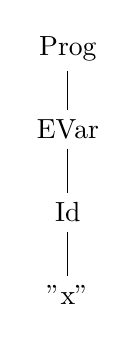
\begin{tikzpicture}
\Tree[.Prog [.EVar [.Id [."x" ]]]]
\end{tikzpicture}
\hfil

\newpage
\begin{lstlisting}[language=Haskell]
-- x x
x x
Prog (EApp (EVar (Id "x")) (EVar (Id "x")))
\end{lstlisting}

\hfil
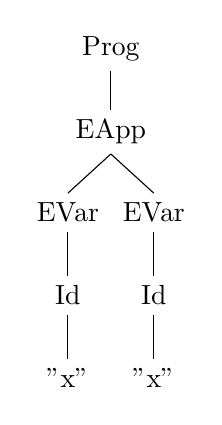
\begin{tikzpicture}
\Tree[.Prog [.EApp [.EVar [.Id [."x" ]]]
                   [.EVar [.Id [."x" ]]]]]
\end{tikzpicture}
\hfil

\begin{lstlisting}[language=Haskell]
-- x y
x y
Prog (EApp (EVar (Id "x")) (EVar (Id "y")))
\end{lstlisting}

\hfil
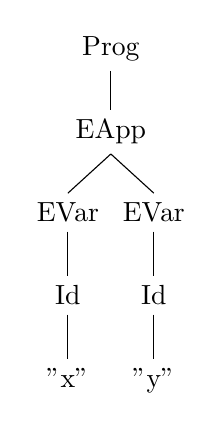
\begin{tikzpicture}
\Tree[.Prog [.EApp [.EVar [.Id [."x" ]]]
                   [.EVar [.Id [."y" ]]]]]
\end{tikzpicture}
\hfil

\begin{lstlisting}[language=Haskell]
-- x y z
x y z
Prog (EApp (EApp (EVar (Id "x")) (EVar (Id "y"))) (EVar (Id "z")))
\end{lstlisting}

\hfil
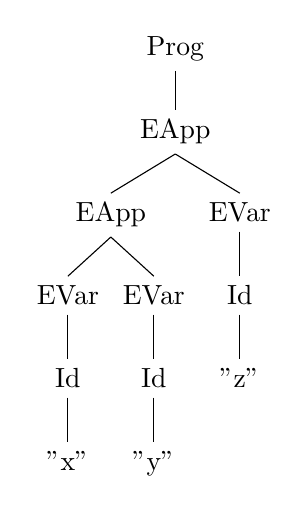
\begin{tikzpicture}
\Tree[.Prog [.EApp [.EApp [.EVar [.Id [."x" ]]]
                          [.EVar [.Id [."y" ]]]]
                   [.EVar [.Id [."z" ]]]]]
\end{tikzpicture}
\hfil

\begin{lstlisting}[language=Haskell]
-- \ x.x
\ x . x
Prog (EAbs (Id "x") (EVar (Id "x")))
\end{lstlisting}

\hfil
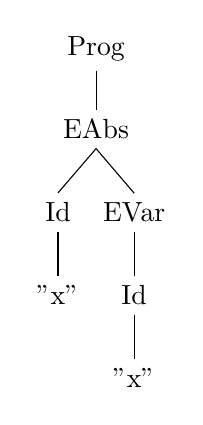
\begin{tikzpicture}
\Tree[.Prog [.EAbs [.Id [."x" ]]
                   [.EVar [.Id [."x" ]]]]]
\end{tikzpicture}
\hfil

\begin{lstlisting}[language=Haskell]
-- \ x.x x
\ x . x x
Prog (EAbs (Id "x") (EApp (EVar (Id "x")) (EVar (Id "x"))))
\end{lstlisting}

\hfil
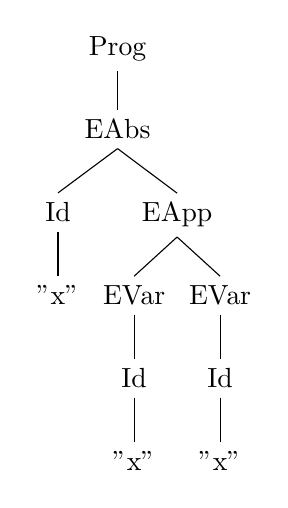
\begin{tikzpicture}
\Tree[.Prog [.EAbs [.Id [."x" ]]
                   [.EApp [.EVar [.Id [."x" ]]]
                          [.EVar [.Id [."x" ]]]]]]
\end{tikzpicture}
\hfil

\newpage
\begin{lstlisting}[language=Haskell]
-- (\ x . (\ y . x y)) (\ x.x) z
\ x . \ y . x y (\ x . x)z
Prog (EApp (EApp (EAbs (Id "x") (EAbs (Id "y") (EApp (EVar (Id "x")) (EVar (Id "y"))))) (EAbs (Id "x") (EVar (Id "x")))) (EVar (Id "z")))
\end{lstlisting}

\hfil
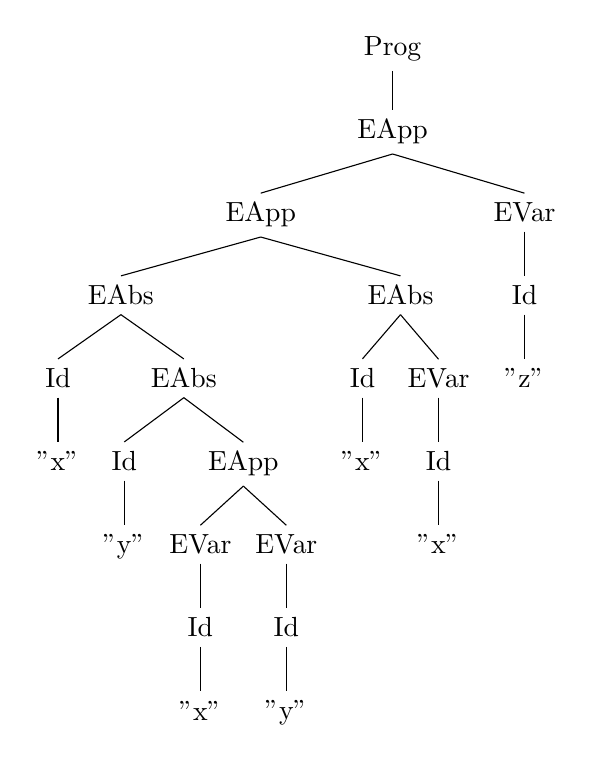
\begin{tikzpicture}
\Tree[.Prog [.EApp [.EApp [.EAbs [.Id [."x" ]]
                                 [.EAbs [.Id [."y" ]]
                                        [.EApp [.EVar [.Id [."x" ]]]
                                               [.EVar [.Id [."y" ]]]]]]
                          [.EAbs [.Id [."x" ]]
                                 [.EVar [.Id [."x" ]]]]]
                   [.EVar [.Id [."z" ]]]]]
\end{tikzpicture}
\hfil

\newpage
\begin{lstlisting}[language=Haskell]
-- (\ x . \ y . x y z) a b c
\ x . \ y . x y z a b c
Prog (EApp (EApp (EApp (EAbs (Id "x") (EAbs (Id "y") (EApp (EApp (EVar (Id "x")) (EVar (Id "y"))) (EVar (Id "z"))))) (EVar (Id "a"))) (EVar (Id "b"))) (EVar (Id "c")))
\end{lstlisting}

\hfil
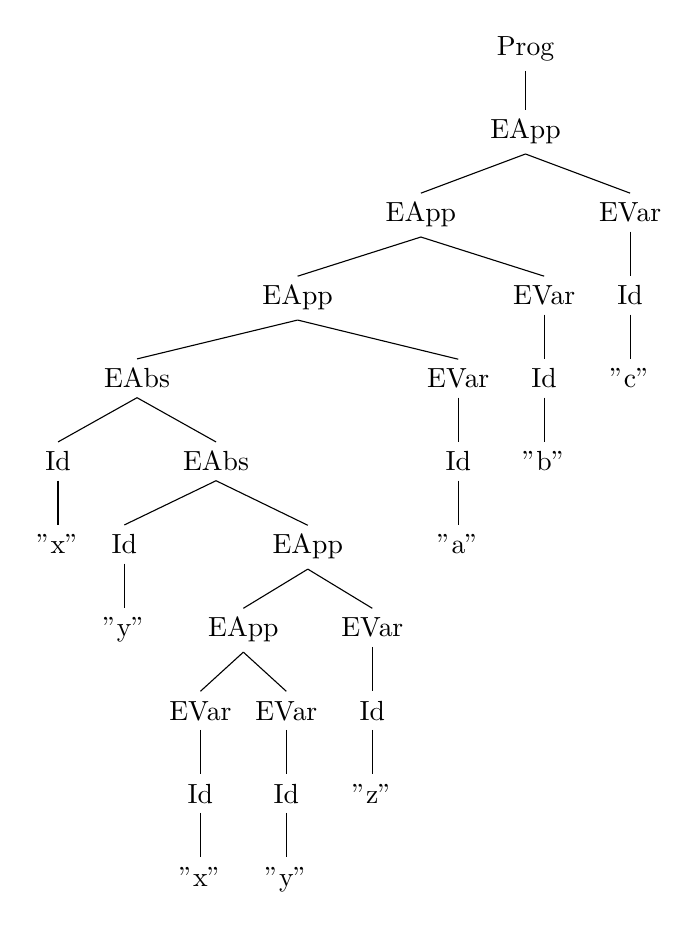
\begin{tikzpicture}
\Tree[.Prog [.EApp [.EApp [.EApp [.EAbs [.Id [."x" ]]
                                        [.EAbs [.Id [."y" ]]
                                               [.EApp [.EApp [.EVar [.Id [."x" ]]]
                                                             [.EVar [.Id [."y" ]]]]
                                                      [.EVar [.Id [."z" ]]]]]]
                                 [.EVar [.Id [."a" ]]]]
                          [.EVar [.Id [."b" ]]]]
                   [.EVar [.Id [."c" ]]]]]
\end{tikzpicture}
\hfil

\noindent The following will show the reduction of several lambda calculus expressions.
\begin{lstlisting}[language=Haskell]
(\x.x) a =
    a
\end{lstlisting}
\begin{lstlisting}[language=Haskell]
\x.x a =
    \x.x a
\end{lstlisting}
\begin{lstlisting}[language=Haskell]
(\x.\y.x) a b =
    (\y.a) b =
    a
\end{lstlisting}
\begin{lstlisting}[language=Haskell]
(\x.\y.y) a b =
    (\y.y) b =
    b
\end{lstlisting}
\newpage
\begin{lstlisting}[language=Haskell]
(\x.\y.x) a b c =
    (\y.a) b c =
    a c
\end{lstlisting}
\begin{lstlisting}[language=Haskell]
(\x.\y.y) a b c =
    (\y.a) b c =
    b c
\end{lstlisting}
\begin{lstlisting}[language=Haskell]
(\x.\y.x) a (b c) =
    (\y.a) (b c) =
    a
\end{lstlisting}
\begin{lstlisting}[language=Haskell]
(\x.\y.y) a (b c) =
    (\y.y) (b c) =
    b c
\end{lstlisting}
\begin{lstlisting}[language=Haskell]
(\x.\y.x) (a b) c =
    (\y.(a b)) c =
    a b
\end{lstlisting}
\begin{lstlisting}[language=Haskell]
(\x.\y.y) (a b) c =
    (\y.y) c =
    c
\end{lstlisting}
\begin{lstlisting}[language=Haskell]
(\x.\y.x) (a b c) =
    \y.(a b c)
\end{lstlisting}
\begin{lstlisting}[language=Haskell]
(\x.\y.y) (a b c) =
    \y.y
\end{lstlisting}
\begin{lstlisting}[language=Haskell]
evalCBN (\x.x)((\y.y)a) =
    evalCBN (EApp (EAbs (Id "x") (EVar (Id "x"))) (EApp (EAbs (Id "y") (EVar (Id "y"))) (EVar (Id "a")))) = -- converted to concrete format
    evalCBN (subst (Id "x") (EApp (EAbs (Id "y") (EVar (Id "y"))) (EVar (Id "a"))) (EVar (Id "x"))) = -- line 27
    evalCBN (EApp (EAbs (Id "y") (EVar (Id "y"))) (EVar (Id "a"))) = -- reduction of subst in one step
    evalCBN (subst (Id "y") (EVar (Id "a")) (EVar (Id "y"))) = -- line 27
    EVar (Id "a") -- reduction of subst in one step
\end{lstlisting}
\newpage
\subsection{Week 6}
The following is an evaluation of a longer lambda calculus expression.

\begin{lstlisting}[language=Haskell]
-- (\exp . \two . \three . exp two three)
-- (\m.\n. m n)
-- (\f.\x. f (f x))
-- (\f.\x. f (f (f x)))

    = ((\m.\n. m n) (\f.\x. f (f x)) (\f.\x. f (f (f x))))
    = ((\m.\n. m n) (\f.\x. f (f x)) (\f2.\x2. f2 (f2 (f2 x2))))
    = ((\n. (\f.\x. f (f x)) n) (\f2.\x2. f2 (f2 (f2 x2))))
    = ((\f.\x. f (f x)) (\f2.\x2. f2 (f2 (f2 x2))))
    = (\x. (\f2.\x2. f2 (f2 (f2 x2))) ((\f2.\x2. f2 (f2 (f2 x2))) x))
    = (\x. (\x2. ((\f2.\x2. f2 (f2 (f2 x2))) x) (((\f2.\x2. f2 (f2 (f2 x2))) x) (((\f2.\x2. f2 (f2 (f2 x2))) x) x2))))
    = (\x. (\x2. (x (x (x (((\f2.\x2. f2 (f2 (f2 x2))) x) (((\f2.\x2. f2 (f2 (f2 x2))) x) x2)))))))
    = (\x. (\x2. (x (x (x (((\x2. x (x (x x2)))) (((\f2.\x2. f2 (f2 (f2 x2))) x) x2)))))))
    = (\x. (\x2. (x (x (x ((\x2. x (x (x x2))) (((\f2.\x2. f2 (f2 (f2 x2))) x) x2)))))))
    = (\x. (\x2. (x (x (x (x (x (x (((\f2.\x2. f2 (f2 (f2 x2))) x) x2)))))))))
    = (\x. (\x2. (x (x (x (x (x (x ((\x2. x (x (x x2))) x2)))))))))
    = \x. \x2. x (x (x (x (x (x (x (x (x x2))))))))
\end{lstlisting}
\subsection{Week 7}
This section will investigate bound and free variables in a lambda-calculus interpreter.

\noindent The following is a section of the interpreter code.
\begin{lstlisting}[language=Haskell]
evalCBN (EApp e1 e2) = case (evalCBN e1) of -- line 5
(EAbs i e3) -> evalCBN (subst i e2 e3)           -- line 6
e3 -> EApp e3 e2                                 -- line 7
\end{lstlisting}

\noindent In this code, all variables (\texttt{e1}, \texttt{e2}, \texttt{e3}, and \texttt{i}) are \textbf{bound variables}. This is because the variable names can be changed without changing the function \texttt{evalCBN}.\newline

\noindent \texttt{e1}:

Binder: \texttt{EApp e1 e2}

Scope: \texttt{case (evalCBN e1) of
| (EAbs i e3) -> evalCBN (subst i e2 e3)
| e3 -> EApp e3 e2}

\noindent \texttt{e2}:

Binder: \texttt{EApp e1 e2}

Scope: \texttt{case (evalCBN e1) of
| (EAbs i e3) -> evalCBN (subst i e2 e3)
| e3 -> EApp e3 e2}

\noindent \texttt{e3}:

Binder (line 6): \texttt{EAbs i e3}

Scope (line 6): \texttt{subst i e2 e3}

Binder (line 7): \texttt{e3}

Scope (line 7): \texttt{EApp e3 e2}

\noindent \texttt{i}:

Binder: \texttt{EAbs i e3}

Scope: \texttt{subst i e2 e3}

\newpage

The following is another section of the interpreter code.
\begin{lstlisting}[language=Haskell]
    subst id s (EAbs id1 e1) =           -- line 18
    let f = fresh (EAbs id1 e1)          -- line 20
        e2 = subst id1 (EVar f) e1 in   -- line 21
        EAbs f (subst id s e2)           -- line 22
\end{lstlisting}

\noindent In this code, all variables (\texttt{id}, \texttt{s}, \texttt{id1}, \texttt{e1}, \texttt{f}, and \texttt{e2}) are \textbf{bound variables}. This is because the variable names can be changed without changing the function \texttt{subst}.\newline

\noindent \texttt{id}:

Binder: \texttt{subst id s (EAbs id1 e1)}

Scope: \texttt{let f = fresh (EAbs id1 e1)
| e2 = subst id1 (EVar f) e1 in
| EAbs f (subst id s e2)}\\

\noindent \texttt{s}:

Binder: \texttt{subst id s (EAbs id1 e1)}

Scope: \texttt{let f = fresh (EAbs id1 e1)
| e2 = subst id1 (EVar f) e1 in
| EAbs f (subst id s e2)}\\

\noindent \texttt{id1}:

Binder: \texttt{EAbs id1 e1}

Scope: \texttt{let f = fresh (EAbs id1 e1)
| e2 = subst id1 (EVar f) e1 in
| EAbs f (subst id s e2)}\\

\noindent \texttt{e1}:

Binder: \texttt{EAbs id1 e1}

Scope: \texttt{let f = fresh (EAbs id1 e1)
| e2 = subst id1 (EVar f) e1 in
| EAbs f (subst id s e2)}\\

\noindent \texttt{f}:

Binder: \texttt{f = fresh (EAbs id1 e1)}

Scope: \texttt{| e2 = subst id1 (EVar f) e1 in
| EAbs f (subst id s e2)}

\noindent \texttt{e2}:

Binder: \texttt{e2 = subst id1 (EVar f) e1}

Scope: \texttt{EAbs f (subst id s e2)}\\

\noindent Another example of evalCBN is demonstrated here:

\begin{lstlisting}[language=Haskell]
evalCBN (\x.\y.x) y z =
    evalCBN (EApp (EApp (EAbs (Id "x") (EAbs (Id "y") (EVar (Id "x")))) (EVar (Id "y"))) (EVar (Id "z"))) = -- converted to concrete format
    evalCBN (EApp (EApp (EAbs (Id "x") (EAbs (Id "y0") (EVar (Id "x")))) (EVar (Id "y"))) (EVar (Id "z"))) = -- fresh applied in one step
    evalCBN (EApp (EApp (evalCBN (subst (Id "y0") (EVar (Id "y")) (EVar (Id "x")))) (EVar (Id "y"))) (EVar (Id "z"))) = -- line 6
    evalCBN (EApp (EAbs (Id "y0") (EVar (Id "y"))) (EVar (Id "z"))) = -- subst reduction
    evalCBN (EApp (evalCBN (subst (Id "y0") (EVar (Id "z")) (EVar (Id "y")))) (EVar (Id "z"))) = -- line 6
    evalCBN (EVar (Id "y")) = -- subst reduction
    EVar (Id "y") -- evalCBN x = x
\end{lstlisting}

The following is an analysis of several abstract reduction systems.

\noindent \texttt{A=\{\}}

A picture will not be drawn for this, for it is just an empty set. This ARS is terminating because it cannot reduce any further. It is confluent because every peak converges to the same result. It has a unique normal form (which is the empty set).\\

\noindent \texttt{A=\{a\} and R=\{\}}

A picture will not be drawn for this, for it is just the letter "a". This ARS is terminating because it cannot reduce any further. It is confluent because every peak converges to the same result. It has a unique normal form (which is "a").\\

\noindent \texttt{A=\{a\} and R=\{(a,a)\}}\\
\begin{center}
    \includegraphics{ars3.png}
\end{center}
This ARS is not terminating because it can always reduce further. It is confluent because every peak converges to the same result. It has a unique normal form (which is "a").\\

\noindent \texttt{A=\{a,b,c\} and R=\{(a,b),(a,c)\}}\\
\begin{center}
    \includegraphics{ars4.png}
\end{center}
This ARS is terminating because it cannot reduce any further. It is not confluent since the computations do not converge back. It does not have a unique normal form.\\

\noindent \texttt{A=\{a,b\} and R=\{(a,a),(a,b)\}}\\
\begin{center}
    \includegraphics{ars5.png}
\end{center}
This ARS is not terminating because it can always reduce further. It is not confluent since the computations do not converge back. It does not have a unique normal form.\\

\noindent \texttt{A=\{a,b,c\} and R=\{(a,b),(b,b),(a,c)\}}\\
\begin{center}
    \includegraphics{ars6.png}
\end{center}
This ARS is not terminating because it can always reduce further. It is not confluent since the computations do not converge back. It does not have a unique normal form.\\

\noindent \texttt{A=\{a,b,c\} and R=\{(a,b),(b,b),(a,c),(c,c)\}}\\
\begin{center}
    \includegraphics{ars7.png}
\end{center}
This ARS is not terminating because it can always reduce further. It is not confluent since the computations do not converge back. It does not have a unique normal form.
\newpage
Lastly, the 8 different cases of confluence, termination, and presence of unique normal forms will be shown.

True, True, True:
\begin{center}
    \includegraphics{ex1.png}
\end{center}

True, True, False: Congruence implies that there are unique normal forms, so there is no example of this case.\\

True, False, True:
\begin{center}
    \includegraphics{ex3.png}
\end{center}

True, False, False: Congruence implies that there are unique normal forms, so there is no example of this case.\\

False, True, True:
\begin{center}
    \includegraphics{ex5.png}
\end{center}

False, True, False:
\begin{center}
    \includegraphics{ex6.png}
\end{center}

False, False, True:
\begin{center}
    \includegraphics{ex7.png}
\end{center}

False, False, False:
\begin{center}
    \includegraphics{ex8.png}
\end{center}
\newpage
\subsection{Week 8}
The following will investigate properties of the following rewrite system:
\begin{lstlisting}
aa -> a
bb -> b
ba -> ab
ab -> ba
\end{lstlisting}

\noindent \textbf{Termination: } This ARS does not terminate because of the final two rules. There is a cycle between the strings \texttt{ab} and \texttt{ba}, meaning that there is no end to the cycle if there exists either of these strings.\\

\noindent \textbf{Normal forms: } The normal forms of this ARS are therefore an empty string, \texttt{a}, and \texttt{b}. Any string longer than one character with just \texttt{ab} and \texttt{ba} will be rewritten as another same-length string, as per the rewrite rules.\\

\noindent \textbf{Unique normal forms: } These rewrite rules can be slightly altered so that the ARS can be defined as having unique normal forms. If we treat \texttt{a} and \texttt{b} as the base-10 digits \texttt{0} and \texttt{1}, it has a slightly different meaning. Because base-10 numbers inherently have an order (0 before 1), these new rewrite rules will allow constant reduction to a normal form not by length, but by number size.\\

\noindent \textbf{ARS function: } The normal forms of this updated rewrite system would thus be the lowest number possible that can be reduced from the starting string. In terms of \texttt{a} and \texttt{b}, the resulting string would have all \texttt{a}'s to the left and all \texttt{b}'s to the right. However, this letter form does not have much meaning, as the letters do not have a predefined comparison order, and thus cannot be counted as a normal form. The normal forms in terms of \texttt{0} and \texttt{1} has more meaning.
\subsection{Week 9}
Regarding the final project, the following deadlines will be made to keep track of progress of my programming language exploration:\\

\noindent \textbf{November 13}: Demonstrate full knowledge of the Ruby language by having a prototype of a concise Ruby tutorial copmlete.\\

\noindent \textbf{November 20}: Have an idea for the project portion of the report laid out in detail.\\

\noindent \textbf{November 27}: Have said project complete and full within the report.\\

\noindent \textbf{December 4}: Have the critical appraisal completed, and therefore the entirety of the Project section of the report complete.
\newpage
\noindent The next section will involve an analysis of the following ARS:
\begin{lstlisting}
ba -> ab
ab -> ba
ac -> ca
ca -> ac
bc -> cb
cb -> bc
 
aa -> b
ab -> c
ac ->  
bb ->
cb -> a
cc -> b
\end{lstlisting}

\noindent The first thing to note is that with this current version of the ARS, it is not terminating, nor does order of the letters matter. This is because the top half of the ARS does not show the entire ARS to be a complete measure function, and that any combination of letters can be reoriented within the entire string. \\

\noindent Also to note are some normal forms, which include the empty string (from Rules 9 and 10) and the one-character strings (\texttt{a}, \texttt{b}, \texttt{c}). The first thing of notice is that any string larger than 1 character can be reduced to a form without any \texttt{a}s. This is because of the reordering rules. Say we order our string so that all \texttt{a}s appear first, followed by \texttt{b}s and \texttt{c}s. Generally, This would turn every pair of \texttt{a}s into \texttt{b}s, with any lone \texttt{a}s therefore joining with newly created \texttt{b}s to form \texttt{c}s. This observation holds for smaller strings as well, of course including those strings that don't contain \texttt{a} to begin with.\\

\noindent After noticing all strings (except for \texttt{a}) can be reduced to a string without \texttt{a}s, I noticed that if the resulting string has an even number of \texttt{b}s and $C mod 4 == 0$ (where C is the number of \texttt{c}s in the string), then the string will reduce to an empty string. This is dependent on Rule 10 and Rule 12, saying that if all \texttt{c}s eventually reduce to an even number of \texttt{b}s, and there were originally an even number of \texttt{b}s already present in the string, then everything will reduce to an empty string.

\subsection{Week 10}
The following is a calculation of $fix_F 2$ using equational reasoning.

\begin{lstlisting}[language=Haskell]
fix_F 2 = (\n. if n == 0 then 1 else n * fix_F (n-1)) 2
         = if 2 == 0 then 1 else 2 * fix_F (2-1)
         = 2 * (fix_F 1)
         = 2 * (\n. if n == 0 then 1 else n * fix_F (n-1)) 1
         = 2 * (if 1 == 0 then 1 else 1 * fix_F (1-1))
         = 2 * (1 * fix_F 0)
         = 2 * (1 * (\n. if n == 0 then 1 else n * fix_F (n-1)) 0)
         = 2 * (1 * (if 0 == 0 then 1 else 0 * fix_F (0-1)))
         = 2 * (1 * (1))
         = 2
\end{lstlisting}


\section{Project}
This section will contain all details for my final project of this course.
\subsection{Specification}
For my final project, I plan to learn a new programming language, give a concise but informative tutorial on it, and develop a project that ties in to the course material. For this, I plan to learn Ruby. Learning a new popular language could be beneficial for personal purposes. My goal is to both learn a relevant language and utilize some concepts learned in the course to create a meaningful project that represents my knowledge of programming languages. The representative project of choice will be determined in the near future.


\section{Conclusions}\label{conclusions}

To be written at a later date.

\end{document}